\documentclass{article}
\usepackage{graphicx}
\usepackage[utf8]{inputenc}
\usepackage{latexsym,amsfonts,amssymb,amsthm,amsmath}
\usepackage[a4paper,margin=1in]{geometry} % Adjust margins as needed
\usepackage{float}
\usepackage{hyperref}
\usepackage{caption}


\setlength{\parindent}{0in}
\setlength{\oddsidemargin}{0in}
\setlength{\textwidth}{6.5in}
\setlength{\textheight}{8.8in}
\setlength{\topmargin}{0in}
\setlength{\headheight}{18pt}




\begin{document}

	\begin{titlepage}
    	\vspace*{\fill} % Add space before the title block
    	\begin{center}
        	{\huge \textbf{CMU Fall24 16820 Homework 5} \par}
       		\vspace{0.5cm}
        		{\large Patrick Chen \par}
        		\vspace{0.5cm}
		%{\large Collaborators: NA \par}
		%\vspace{0.5cm}
        		{\large November 10, 2024 \par}
    	\end{center}
    	\vspace*{\fill} % Add space after the title block to center everything
	\end{titlepage}
	
	\newpage
	\subsection*{Q1-a at page 3}
	Ans:\\
	\hangindent=1.5em \hspace{1.5em}According to Lambertian's cosine law, the intensity of light observed from a Lambertian surface is propational to the cosine of the angle $\theta$ between the surface normal, $\vec{n}$, and the direction of the incoming light, $\vec{l}$.
	\begin{align}
		\mathbf{\overrightarrow{n}} \cdot \mathbf{\overrightarrow{l}} = |\mathbf{\overrightarrow{n}}| |\mathbf{\overrightarrow{l}}| \cos(\theta) 
	\end{align}
	Typically in the context of n-dot-l lighting, both $\vec{n}$ and $\vec{l}$ are unit vectors, so we have:
	\begin{align}
	\mathbf{\overrightarrow{n}} \cdot \mathbf{\overrightarrow{l}} = \cos(\theta) 
	\end{align}
	As shown in Fig. 2a as below, the $\theta$ is the dot product between $\vec{n}$ and $\vec{l}$. The dot product, $\theta$, quantifies the amount of incident light that is effectively contributing to the brightness of the surface. As the angle increases, less light is effectively reaching the surface, as the angle decrease, more light hits the surface, reaching maximum incoming light when $\theta$ is 0, identical to the case that $\vec{l}$ is aligned with $\vec{n}$.
	
	\begin{minipage}{0.48\linewidth}
	\centering
	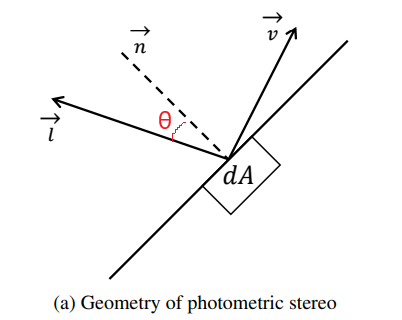
\includegraphics[width=\linewidth]{./Q1_a.png}
	\refstepcounter{figure}  % Increment the figure counter
	\textbf{Fig. 2a} % Manually add a caption/title
	\label{fig:Q1_a}         % Label for referencing	
	\end{minipage}
	\hfill
	\begin{minipage}{0.48\linewidth}
	\centering
	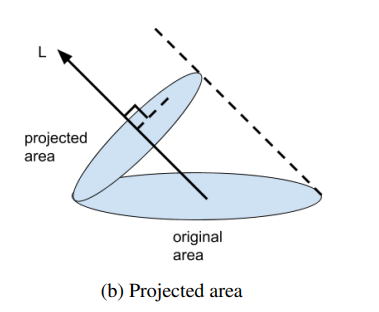
\includegraphics[width=\linewidth]{./Q1_b.png}
	\refstepcounter{figure}  % Increment the figure counter
	\textbf{Fig. 2b} % Manually add a caption/title
	\label{fig:Q1_b}         % Label for referencing
	\end{minipage}	
	\newline
	
	\hangindent=1.5em \hspace{1.5em}The projected area, $\mathbf{dA_{projected}}$, in Fig. 2b is the original area, $\mathbf{dA}$, times $\cos(\theta)$:
	\begin{align}
		\mathbf{dA_{projected}} &= \mathbf{dA} \cdot \cos(\theta) \\
								&= \mathbf{dA} \cdot \mathbf{\overrightarrow{n}} \cdot \mathbf{\overrightarrow{l}} \\
		\frac{\mathbf{dA_{projected}}}{\mathbf{dA}} &= \cos(\theta) \\
													&= \mathbf{\overrightarrow{n}} \cdot \mathbf{\overrightarrow{l}}
	\end{align}
	As $\theta$ becomes larger, the effective area that light directly expose to becomes smaller, and on the opposite, as $\theta$ becomes smaller, the effective area becomes larger, reaching maximum $\mathbf{dA}$ as $\theta$ = 0. Hence, the projected area comes into the equation as part of the Lambertian reflectance model through the $\cos(\theta)$ factor.
	\newline
	
	\hangindent=1.5em \hspace{1.5em}The reason that the viewing direction does not matter is that we assume the surface is Lambertial surface, which reflects light equally in all directions, $\vec{v}$. Specifically, the light reflected from each point on the surface has the same intensity value no matter where the observer is located. It also means that the intensity of light that the observer can observe is based solely on the $\vec{n} \cdot \vec{l} = \cos(\theta)$ term.

	\newpage
	
	\newpage
	\subsection*{Q1-b at page 4}
	Ans:\\
	\hangindent=1.5em \hspace{1.5em}Following \autoref{fig:Q1_b_a} - \autoref{fig:Q1_b_c} shows the rendered result, and the \autoref{fig:Q1_b_cns} shows the code snippet in q1.py.
	\newline
	
	\begin{minipage}{0.31\linewidth}
	\centering
	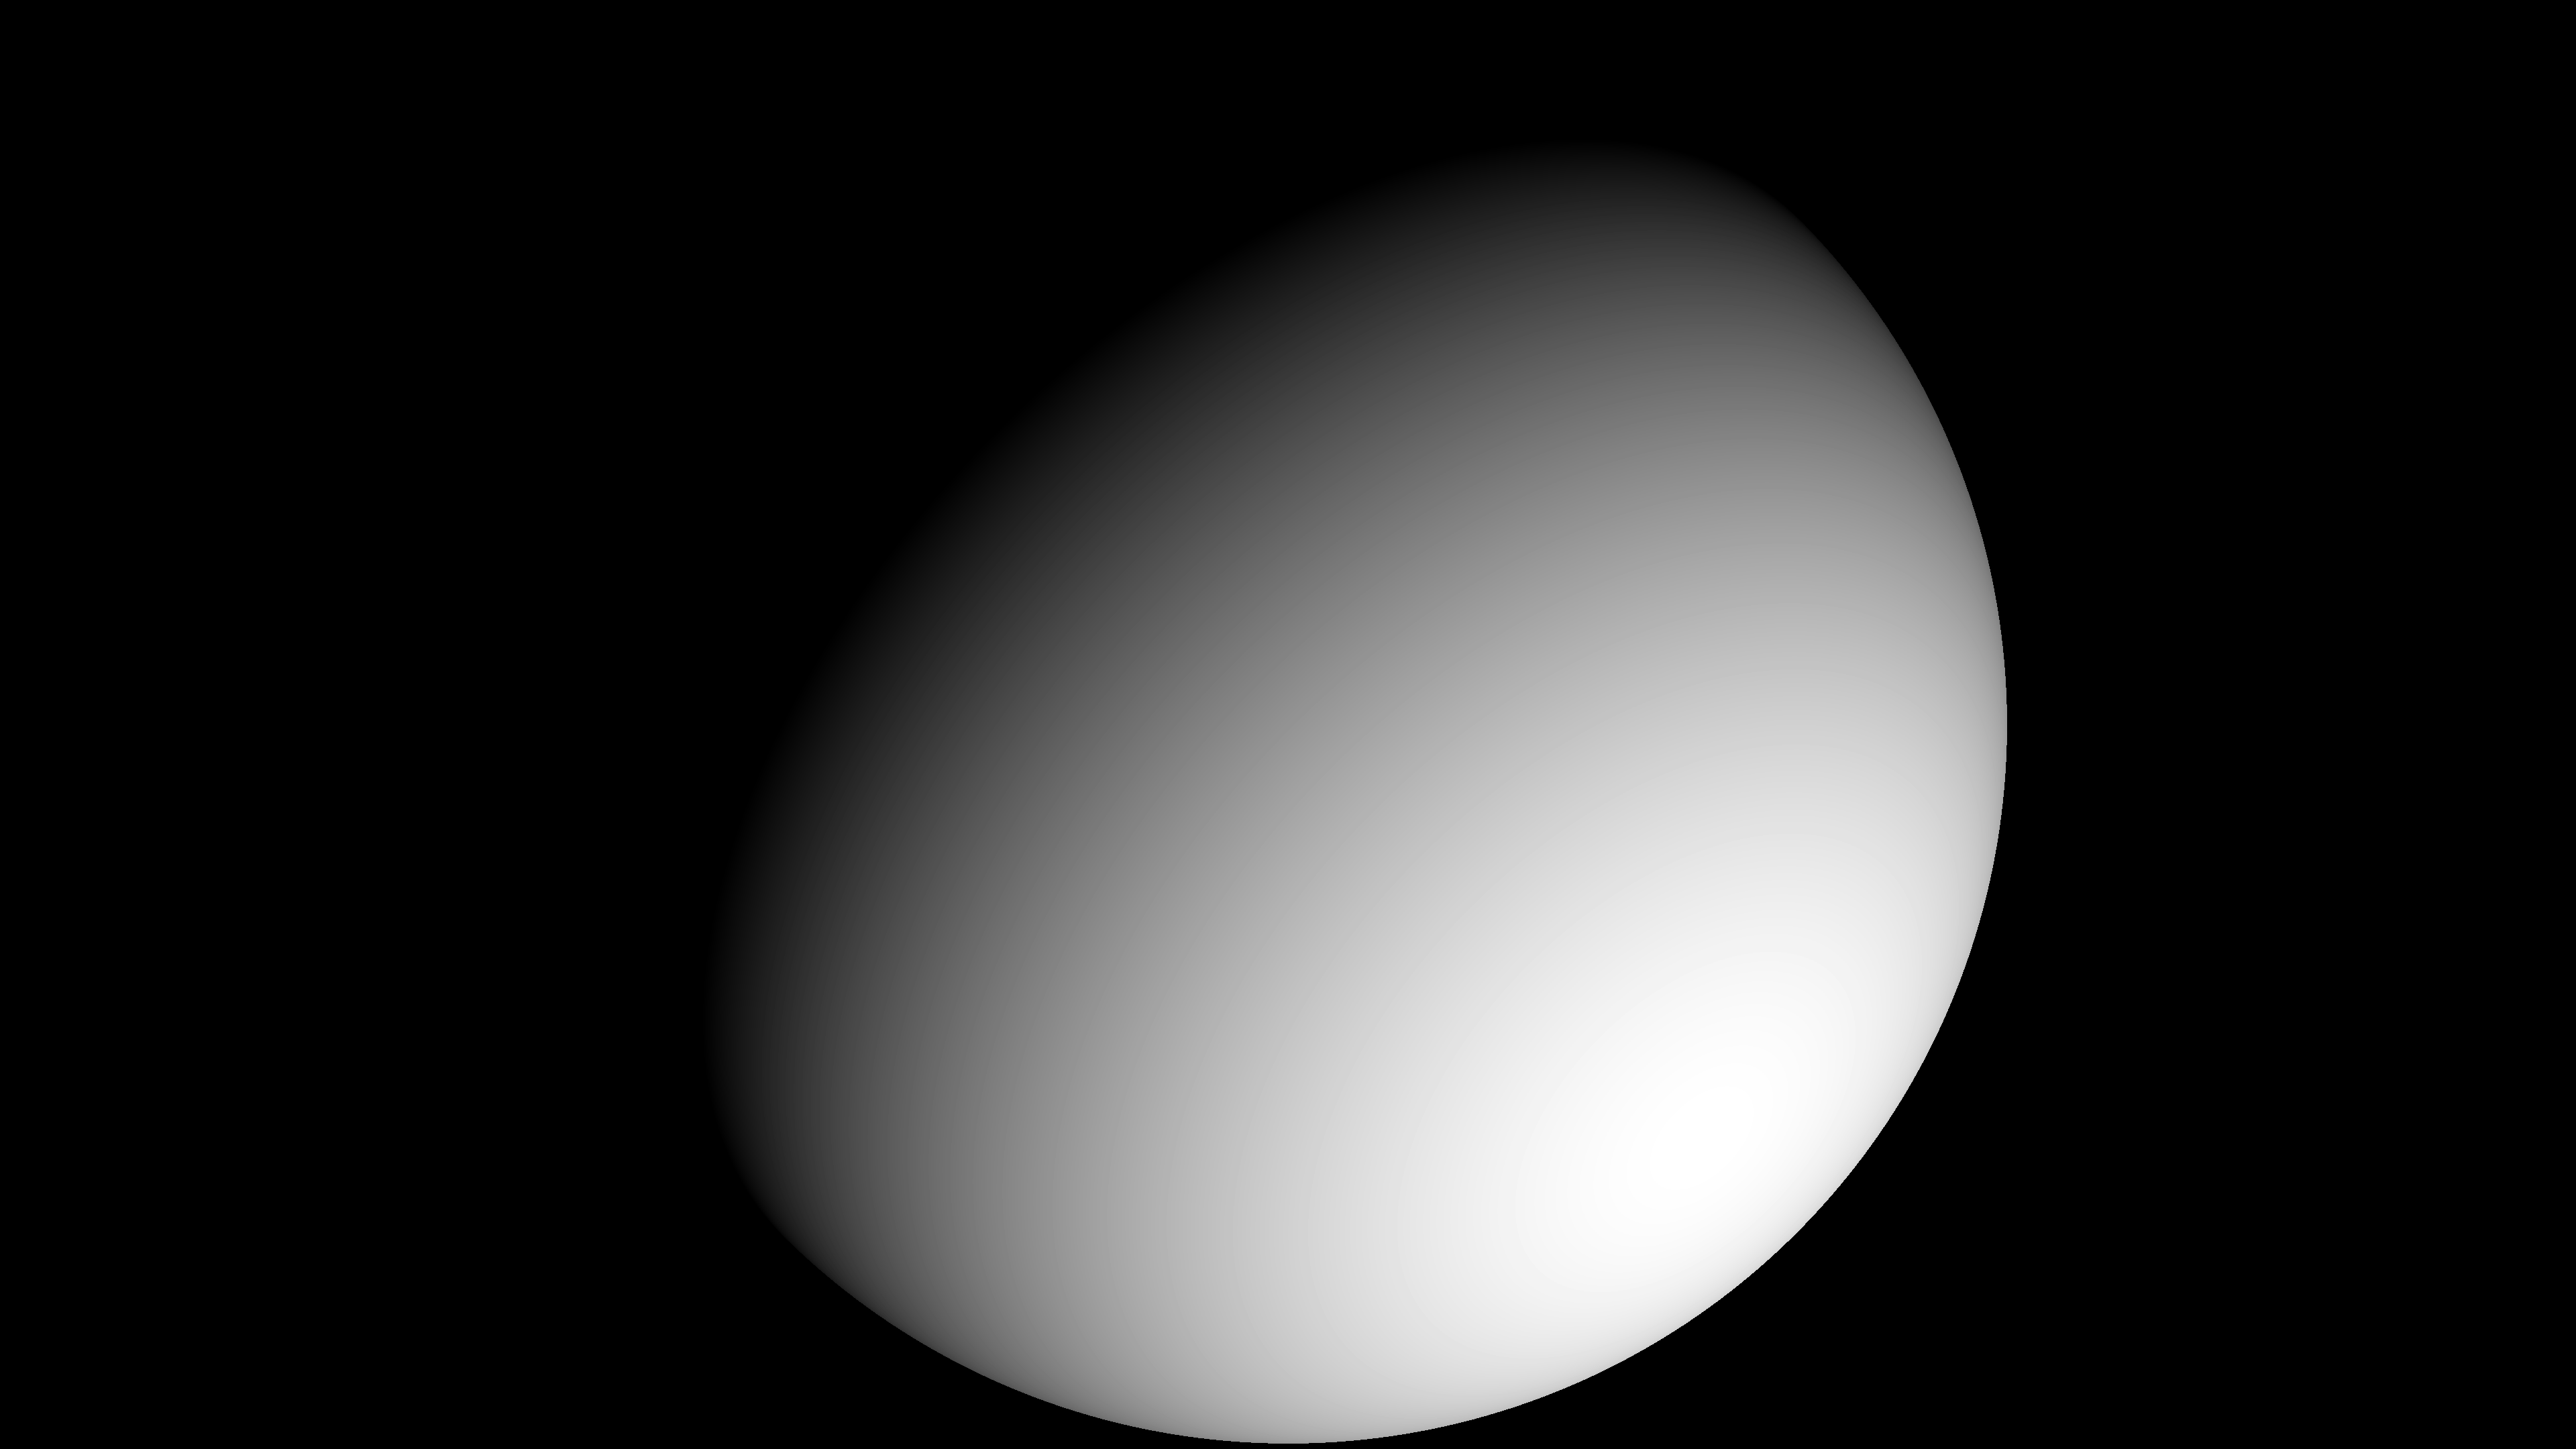
\includegraphics[width=\linewidth]{./src/1b-a.png}
	\refstepcounter{figure}  % Increment the figure counter
	\textbf{Figure \thefigure:} Rendered Result with (1, 1, 1)/$\sqrt{3}$ Light Vector  % Manually add a caption/title
	\label{fig:Q1_b_a}         % Label for referencing	
	\end{minipage}
\hfill
	\begin{minipage}{0.31\linewidth}
	\centering
	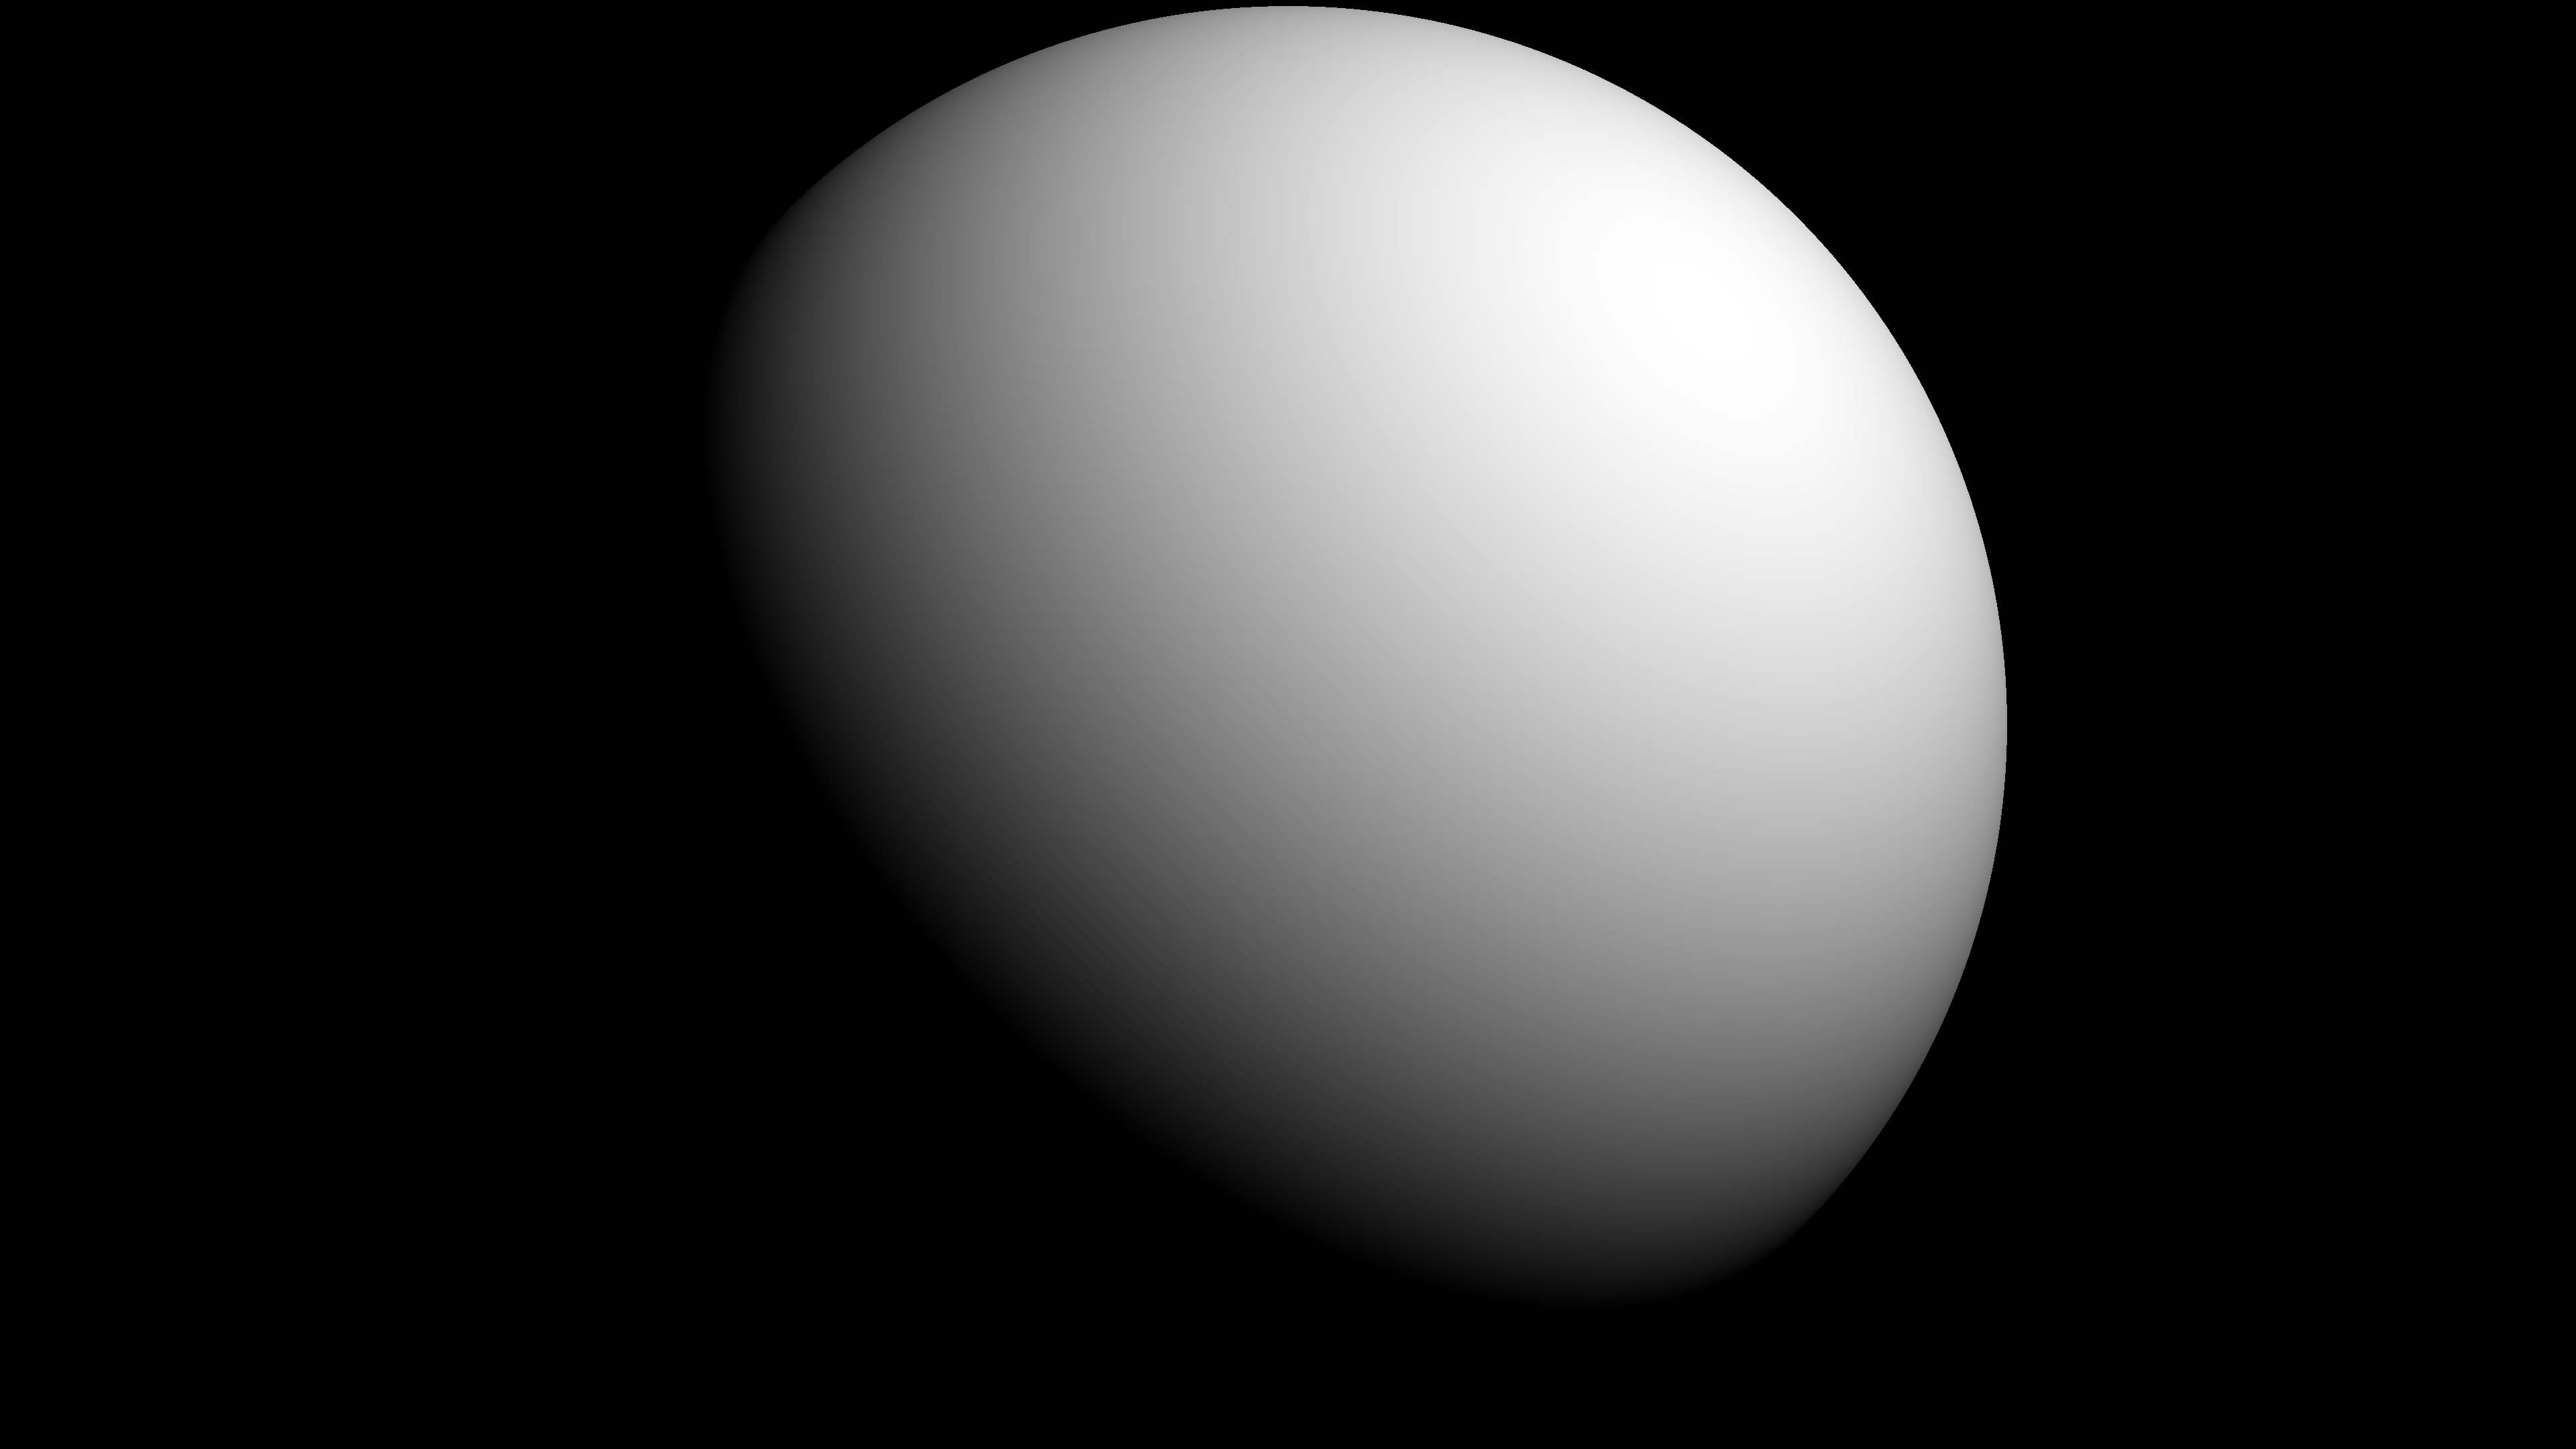
\includegraphics[width=\linewidth]{./src/1b-b.png}
	\refstepcounter{figure}  % Increment the figure counter
	\textbf{Figure \thefigure:} Rendered Result with (1, -1, 1)/$\sqrt{3}$ Light Vector  % Manually add a caption/title
	\label{fig:Q1_b_b}         % Label for referencing
	\end{minipage}	
\hfill
	\begin{minipage}{0.31\linewidth}
	\centering
	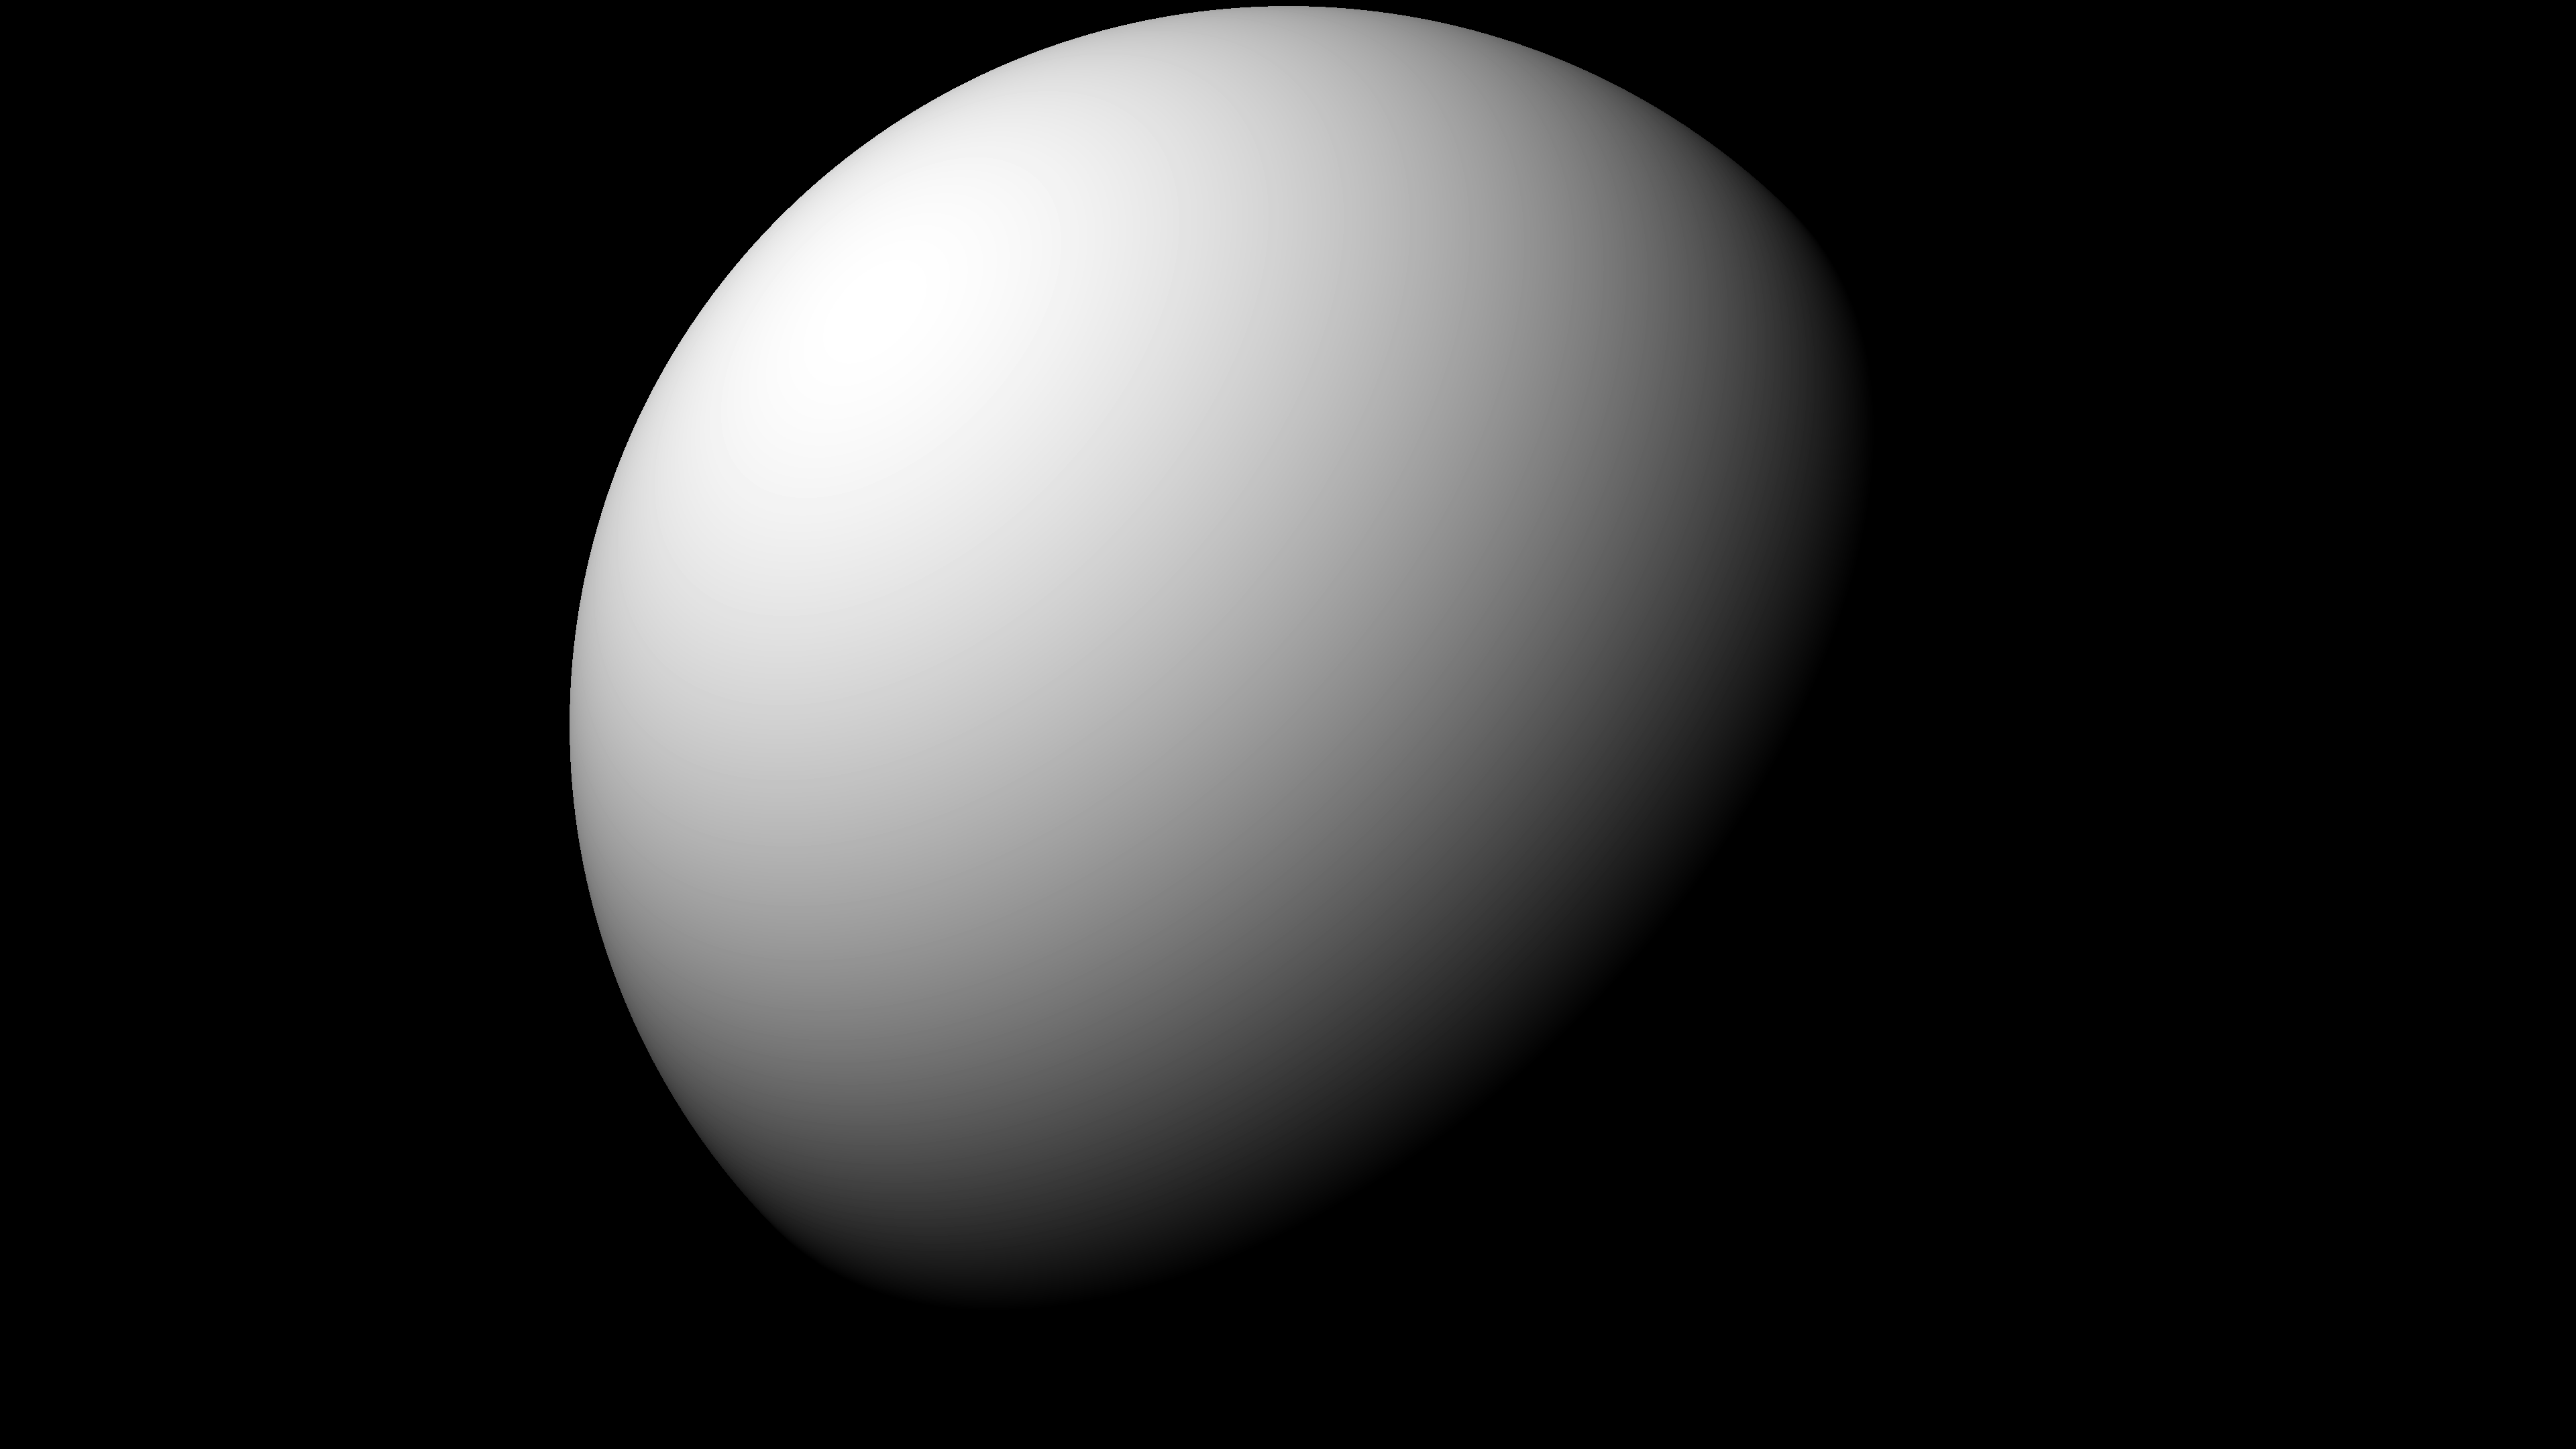
\includegraphics[width=\linewidth]{./src/1b-c.png}
	\refstepcounter{figure}  % Increment the figure counter
	\textbf{Figure \thefigure:} Rendered Result with (-1, -1, 1)/$\sqrt{3}$ Light Vector  % Manually add a caption/title
	\label{fig:Q1_b_c}         % Label for referencing
	\end{minipage}	
	\newline
	\newline

	\begin{minipage}{1\linewidth}
	\centering
	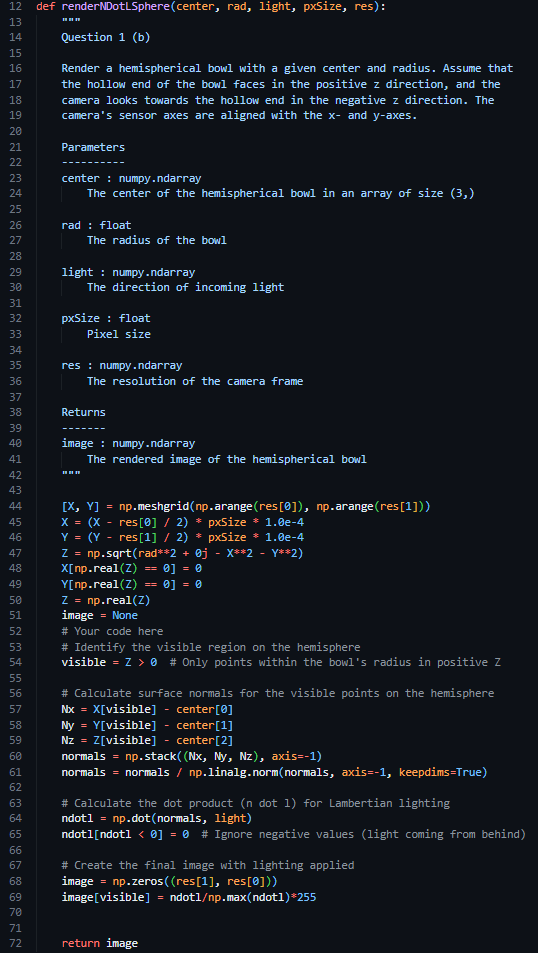
\includegraphics[width=0.7\linewidth, height=0.95\columnwidth]{./Q1_b_cns.png}
	\refstepcounter{figure}  \\% Increment the figure counter
	\textbf{Figure \thefigure:} Code Snippet  % Manually add a caption/title
	\label{fig:Q1_b_cns}         % Label for referencing
	\end{minipage}	
	
	\newpage
	\subsection*{Q1-c at page 4}
	Ans:\\
	\hangindent=1.5em \hspace{1.5em}Following.
	\newline


	\newpage
	\subsection*{Collaborations}
	Ans:\\
	\hangindent=0.4em \hspace{0.3em} Though I do not have collaborators, I found the following websites helpful on understanding the concepts in this homework.
	\begin{enumerate}
		\item \url{https://www.ri.cmu.edu/pub_files/pub3/baker_simon_2003_3/baker_simon_2003_3.pdf.}
		\item \url{https://pytorch.org/tutorials/beginner/pytorch_with_examples.html}
		\item \url{https://matplotlib.org/stable/api/_as_gen/matplotlib.pyplot.imsave.html}	
		\item \url{https://www.geeksforgeeks.org/how-to-load-cifar10-dataset-in-pytorch/}	
		\item \url{https://www.geeksforgeeks.org/how-do-you-use-pytorchs-dataset-and-dataloader-classes-for-custom-data/}
		\item \url{https://github.com/facebookarchive/fb.resnet.torch/issues/180}
		\item \url{https://pytorch.org/tutorials/beginner/data_loading_tutorial.html#afterword-torchvision}
		\item \url{https://www.kaggle.com/code/satriasyahputra/flowers-17}
	\end{enumerate}

\end{document}